% * Latex header
% ** Document class
\documentclass[10pt,letterpaper]{article}\usepackage[]{graphicx}\usepackage[]{color}
%% maxwidth is the original width if it is less than linewidth
%% otherwise use linewidth (to make sure the graphics do not exceed the margin)
\makeatletter
\def\maxwidth{ %
  \ifdim\Gin@nat@width>\linewidth
    \linewidth
  \else
    \Gin@nat@width
  \fi
}
\makeatother

\definecolor{fgcolor}{rgb}{0.345, 0.345, 0.345}
\newcommand{\hlnum}[1]{\textcolor[rgb]{0.686,0.059,0.569}{#1}}%
\newcommand{\hlstr}[1]{\textcolor[rgb]{0.192,0.494,0.8}{#1}}%
\newcommand{\hlcom}[1]{\textcolor[rgb]{0.678,0.584,0.686}{\textit{#1}}}%
\newcommand{\hlopt}[1]{\textcolor[rgb]{0,0,0}{#1}}%
\newcommand{\hlstd}[1]{\textcolor[rgb]{0.345,0.345,0.345}{#1}}%
\newcommand{\hlkwa}[1]{\textcolor[rgb]{0.161,0.373,0.58}{\textbf{#1}}}%
\newcommand{\hlkwb}[1]{\textcolor[rgb]{0.69,0.353,0.396}{#1}}%
\newcommand{\hlkwc}[1]{\textcolor[rgb]{0.333,0.667,0.333}{#1}}%
\newcommand{\hlkwd}[1]{\textcolor[rgb]{0.737,0.353,0.396}{\textbf{#1}}}%
\let\hlipl\hlkwb

\usepackage{framed}
\makeatletter
\newenvironment{kframe}{%
 \def\at@end@of@kframe{}%
 \ifinner\ifhmode%
  \def\at@end@of@kframe{\end{minipage}}%
  \begin{minipage}{\columnwidth}%
 \fi\fi%
 \def\FrameCommand##1{\hskip\@totalleftmargin \hskip-\fboxsep
 \colorbox{shadecolor}{##1}\hskip-\fboxsep
     % There is no \\@totalrightmargin, so:
     \hskip-\linewidth \hskip-\@totalleftmargin \hskip\columnwidth}%
 \MakeFramed {\advance\hsize-\width
   \@totalleftmargin\z@ \linewidth\hsize
   \@setminipage}}%
 {\par\unskip\endMakeFramed%
 \at@end@of@kframe}
\makeatother

\definecolor{shadecolor}{rgb}{.97, .97, .97}
\definecolor{messagecolor}{rgb}{0, 0, 0}
\definecolor{warningcolor}{rgb}{1, 0, 1}
\definecolor{errorcolor}{rgb}{1, 0, 0}
\newenvironment{knitrout}{}{} % an empty environment to be redefined in TeX

\usepackage{alltt}
% ** Packages
\usepackage[top=0.85in]{geometry}
\usepackage{amsmath,amssymb}
\usepackage{changepage}
\usepackage[utf8x]{inputenc}
\usepackage{textcomp,marvosym}
\usepackage{cite}
\usepackage{nameref,hyperref}
\usepackage[right]{lineno}
\usepackage{microtype}
\usepackage[table]{xcolor}
\usepackage{array}
\usepackage{caption}
\usepackage{adjustbox}
% ** Setting
\DisableLigatures[f]{encoding = *, family = * }
% * Document
% ** Title
\IfFileExists{upquote.sty}{\usepackage{upquote}}{}
\begin{document}
{\Large
  \noindent\textbf{SuperLearner versus Clinicians to Prioritise Trauma Patients (working title)}
} \newline
\\
% ** Version
{\large
  Test version 0.0.0.9000
}
% ** Results
\section*{Results}
During the study period, we approached a total of 1500 patients
for enrollment. 54 patients did
not provide informed consent. Out of the 1446
patients who provided informed consent, 99 had missing data on priority level
assigned by clinicians, leaving 1401
patients. An additional 539 were excluded because of missing outcome
data. Thus, the final study sample included
862 patients.

Table \ref{tab:sample-characteristics} shows sample characteristics. The median
age among included patients was 30 (IQR 24-42) years. A majority,
680 (79\%) patients, were males. The most common mechanism
of injury was transport accidents, accounting for 358 (42\%) patients. A total of 518 (60\%) patients were transported to participating centres in some sort of
private vehicle, such as a car, taxi, or rickshaw. A majority of patients had
normal vital signs on arrival to participating centres. Out of all patients,
61 (7\%) died within 30 days of arrival. The number of
patients in the training and test samples were 562 and
300 respectively.

% latex table generated in R 3.3.3 by xtable 1.8-2 package
% Sun May 20 16:55:05 2018
\begin{table}[ht]
\centering
\caption{Sample characteristics} 
\label{tab:sample-characteristics}
\begin{adjustbox}{max width=\textwidth} 
\begin{tabular} 
{lllll}
  \hline
Characteristic & Level & Training & Test & Overall \\ 
  \hline
n (\%) &  & 562 (65.2) & 300 (34.8) & 862 (100.0) \\ 
  Age in years (median [IQR]) &  & 30.0 [24.0, 45.0] & 30.0 [23.0, 40.0] & 30.0 [24.0, 42.0] \\ 
  Sex (\%) & Female & 117 (20.8) & 65 (21.7) & 182 (21.1) \\ 
   & Male & 445 (79.2) & 235 (78.3) & 680 (78.9) \\ 
  Mechanism of injury (\%) & Assault & 77 (13.7) & 49 (16.3) & 126 (14.6) \\ 
   & Burn & 2 (0.4) & 1 (0.3) & 3 (0.3) \\ 
   & Event of undetermined intent & 1 (0.2) & 0 (0.0) & 1 (0.1) \\ 
   & Fall & 150 (26.7) & 81 (27.0) & 231 (26.8) \\ 
   & Intentional self harm & 2 (0.4) & 1 (0.3) & 3 (0.3) \\ 
   & Other external cause of accidental injury & 67 (11.9) & 73 (24.3) & 140 (16.2) \\ 
   & Transport accident & 263 (46.8) & 95 (31.7) & 358 (41.5) \\ 
  Type of injury (\%) & Blunt & 550 (97.9) & 300 (100.0) & 850 (98.6) \\ 
   & Penetrating & 10 (1.8) & 0 (0.0) & 10 (1.2) \\ 
   & Blunt and penetrating & 2 (0.4) & 0 (0.0) & 2 (0.2) \\ 
  Mode of transport (\%) & Ambulance & 238 (42.3) & 41 (13.7) & 279 (32.4) \\ 
   & Police & 24 (4.3) & 8 (2.7) & 32 (3.7) \\ 
   & Private vehicle & 286 (50.9) & 232 (77.3) & 518 (60.1) \\ 
   & Arrived walking & 14 (2.5) & 19 (6.3) & 33 (3.8) \\ 
  Transferred (\%) & No & 315 (56.0) & 253 (84.3) & 568 (65.9) \\ 
   & Yes & 247 (44.0) & 47 (15.7) & 294 (34.1) \\ 
  SBP (median [IQR]) &  & 120.0 [111.0, 130.0] & 122.0 [114.0, 134.0] & 121.0 [112.0, 132.0] \\ 
  DBP (median [IQR]) &  & 80.0 [70.0, 86.8] & 82.0 [73.0, 90.0] & 80.0 [72.0, 88.0] \\ 
  SpO\textsuperscript{2} (median [IQR]) &  & 98.0 [97.0, 98.0] & 98.0 [98.0, 98.0] & 98.0 [97.0, 98.0] \\ 
  HR (median [IQR]) &  & 88.0 [78.0, 96.8] & 87.0 [78.0, 100.0] & 88.0 [78.0, 98.0] \\ 
  RR (median [IQR]) &  & 20.0 [18.0, 22.0] & 24.0 [20.0, 26.0] & 22.0 [18.0, 24.0] \\ 
  EGCS (\%) & 1 & 33 (5.9) & 11 (3.7) & 44 (5.1) \\ 
   & 2 & 8 (1.4) & 1 (0.3) & 9 (1.0) \\ 
   & 3 & 17 (3.0) & 1 (0.3) & 18 (2.1) \\ 
   & 4 & 503 (89.5) & 286 (95.3) & 789 (91.5) \\ 
   & Non testable & 1 (0.2) & 1 (0.3) & 2 (0.2) \\ 
  VGCS (\%) & 1 & 35 (6.2) & 10 (3.3) & 45 (5.2) \\ 
   & 2 & 11 (2.0) & 4 (1.3) & 15 (1.7) \\ 
   & 3 & 7 (1.2) & 0 (0.0) & 7 (0.8) \\ 
   & 4 & 22 (3.9) & 0 (0.0) & 22 (2.6) \\ 
   & 5 & 487 (86.7) & 285 (95.0) & 772 (89.6) \\ 
   & Non testable & 0 (0.0) & 1 (0.3) & 1 (0.1) \\ 
  MGCS (\%) & 1 & 15 (2.7) & 4 (1.3) & 19 (2.2) \\ 
   & 2 & 7 (1.2) & 2 (0.7) & 9 (1.0) \\ 
   & 3 & 9 (1.6) & 4 (1.3) & 13 (1.5) \\ 
   & 4 & 6 (1.1) & 1 (0.3) & 7 (0.8) \\ 
   & 5 & 23 (4.1) & 3 (1.0) & 26 (3.0) \\ 
   & 6 & 500 (89.0) & 286 (95.3) & 786 (91.2) \\ 
   & Non testable & 2 (0.4) & 0 (0.0) & 2 (0.2) \\ 
  AVPU (\%) & Unresponsive & 17 (3.0) & 4 (1.3) & 21 (2.4) \\ 
   & Pain responsive & 28 (5.0) & 9 (3.0) & 37 (4.3) \\ 
   & Voice responsive & 18 (3.2) & 1 (0.3) & 19 (2.2) \\ 
   & Alert & 499 (88.8) & 286 (95.3) & 785 (91.1) \\ 
  Delay (median [IQR]) &  & 170.0 [50.0, 893.5] & 66.0 [35.0, 288.0] & 120.0 [43.2, 693.8] \\ 
  All cause 30-day mortality (\%) & No & 512 (91.1) & 289 (96.3) & 801 (92.9) \\ 
   & Yes & 50 (8.9) & 11 (3.7) & 61 (7.1) \\ 
   \hline
\end{tabular} 
\end{adjustbox}
\caption*{Abbreviations and explanations: AVPU, Alert, voice, pain, unresponsive scale; DBP, Diastolic blood pressure in mmHg; Delay, Time between injury and arrival to participating centre in minutes; EGCS, Eye component of the Glasgow Coma Scale; HR, Heart rate; MGCS, Motor component of the Glasgow Coma Scale; RR, Respiratory rate in breaths per minute; SBP, Systolic blood pressure in mmHg; SpO\textsuperscript{2}, Peripheral capillary oxygen saturation; Transferred, Transferred from another health facility; VGCS, Verbal component of the Glasgow Coma Scale} 
\end{table}


The AUROCC of the continuous SuperLearner prediction in the training sample was
0.9994 (Figure \ref{fig:roc_plot}A). Figure
\ref{fig:calibration_plot}A shows the agreement between the continuous
predictions and observed outcomes in the training sample. The cutpoints
identified by the grid search were 0.1,
0.28, and 0.73. We used these
cutpoints to bin the continuous SuperLearner prediction into the four priority
levels green, yellow, orange, and red. The AUROCC of the binned SuperLearner
predictions in the training sample was
0.9997. Table \ref{tab:superlearner-train-table}
shows the number of patients and all cause 30-day mortality in each group.

% latex table generated in R 3.3.3 by xtable 1.8-2 package
% Sun May 20 16:09:11 2018
\begin{table}[ht]
\centering
\caption{Priority levels assigned by the binned SuperLearner prediction in the training sample (n = 562)} 
\label{tab:superlearner-priorities-train}
\begin{tabular}{llllll}
  \hline
All cause 30-day mortality & Green (\%) & Yellow (\%) & Orange (\%) & Red (\%) & Overall (\%) \\ 
  \hline
No & 483 (100) & 23 (74) & 6 (35) & 0 (0) & 512 (91) \\ 
  Yes & 0 (0) & 8 (26) & 11 (65) & 31 (100) & 50 (9) \\ 
   \hline
\end{tabular}
\end{table}


We then applied the SuperLearner to the test sample. The AUROCC of the continous
SuperLearner prediction was 0.9811 Figure
\ref{fig:roc_plot}B. Figure \ref{fig:calibration_plot}B shows the agreement
between the continuous predictions and observed outcomes in the test sample. We
used the same cutpoints as in the training sample to bin the continuous
predictions into the four priority levels. The AUROCC of the binned SuperLearner
predictions in the test sample was 0.9429. Table
\ref{tab:superlearner-test-table} shows the number of patients and all cause
30-day mortality in each group. 

% latex table generated in R 3.3.3 by xtable 1.8-2 package
% Sun May 20 16:09:11 2018
\begin{table}[ht]
\centering
\caption{Priority levels assigned by the binned SuperLearner prediction in the test sample (n = 300)} 
\label{tab:superlearner-priorities-test}
\begin{tabular}{llllll}
  \hline
All cause 30-day mortality & Green (\%) & Yellow (\%) & Orange (\%) & Red (\%) & Overall (\%) \\ 
  \hline
No & 279 (100) & 6 (100) & 4 (44) & 0 (0) & 289 (96) \\ 
  Yes & 1 (0) & 0 (0) & 5 (56) & 5 (100) & 11 (4) \\ 
   \hline
\end{tabular}
\end{table}


In the test sample we compared the performance of the binned SuperLearner
prediction with that of clinicians. The AUROCC of priority levels assigned by
clinicians was 0.9723. Table \ref{tab:clinicians-test-table}
shows the priority levels assigned by clinicians and the all cause 30-day
mortality in each group. The difference in AUROCC between the binned
SuperLearner prediction and clinicians was
0.0294 (95\% CI -0.0313 - 0.0672). The net reclassifciation in events and
non-events were 0.0033 (95\% CI 0.0034 - 0.0139) and -0.0133 (95\% CI -0.1321 - -0.1003) respectively. The overall
reclassification is show in Table \ref{tab:reclass_all}. Figure
\ref{fig:mortality_plot} shows the all cause 30-day mortality across priority
levels assigned by the SuperLearner and clinicians.

% latex table generated in R 3.3.3 by xtable 1.8-2 package
% Sun May 20 16:09:11 2018
\begin{table}[ht]
\centering
\caption{Priority levels assigned clinicians in the test sample (n = 300)} 
\label{tab:clinicians-priorities-test}
\begin{tabular}{llllll}
  \hline
All cause 30-day mortality & Green (\%) & Yellow (\%) & Orange (\%) & Red (\%) & Overall (\%) \\ 
  \hline
No & 250 (100) & 32 (91) & 4 (67) & 3 (33) & 289 (96) \\ 
  Yes & 0 (0) & 3 (9) & 2 (33) & 6 (67) & 11 (4) \\ 
   \hline
\end{tabular}
\end{table}


% latex table generated in R 3.3.3 by xtable 1.8-2 package
% Sun May 20 16:09:11 2018
\begin{table}[ht]
\centering
\caption{Priority levels assigned by SuperLearner and clinicians in complete test sample (n = 300)} 
\label{tab:reclass_all}
\begin{tabular}{llllllll}
  \hline
  & \multicolumn{4}{c}{SuperLearner} \\
 Clinicians & Green & Yellow & Orange & Red & Rec. \% & Rec. up \% & Rec. down \% \\
 \hline
Green & 249 & 0 & 1 & 0 & 0 & 0 &  \\ 
  Yellow & 29 & 3 & 2 & 1 & 91 & 9 & 83 \\ 
  Orange & 0 & 3 & 3 & 0 & 50 & 0 & 50 \\ 
  Red & 2 & 0 & 3 & 4 & 56 &  & 56 \\ 
   \hline
\end{tabular}
\caption*{Reclassification (Rec.) figures refer to \% of patients reclassified by the SuperLearner compared to clinicians. Rec. up and Rec. down indicates \% of patients reclassified to a higher or lower priority level respectively.} 
\end{table}


% ** Figures
% *** ROC plots
\begin{figure}
  \caption{Receiver operating characteristics curves in training (A) and test
    (B) samples}
  \label{fig:roc_plot}
  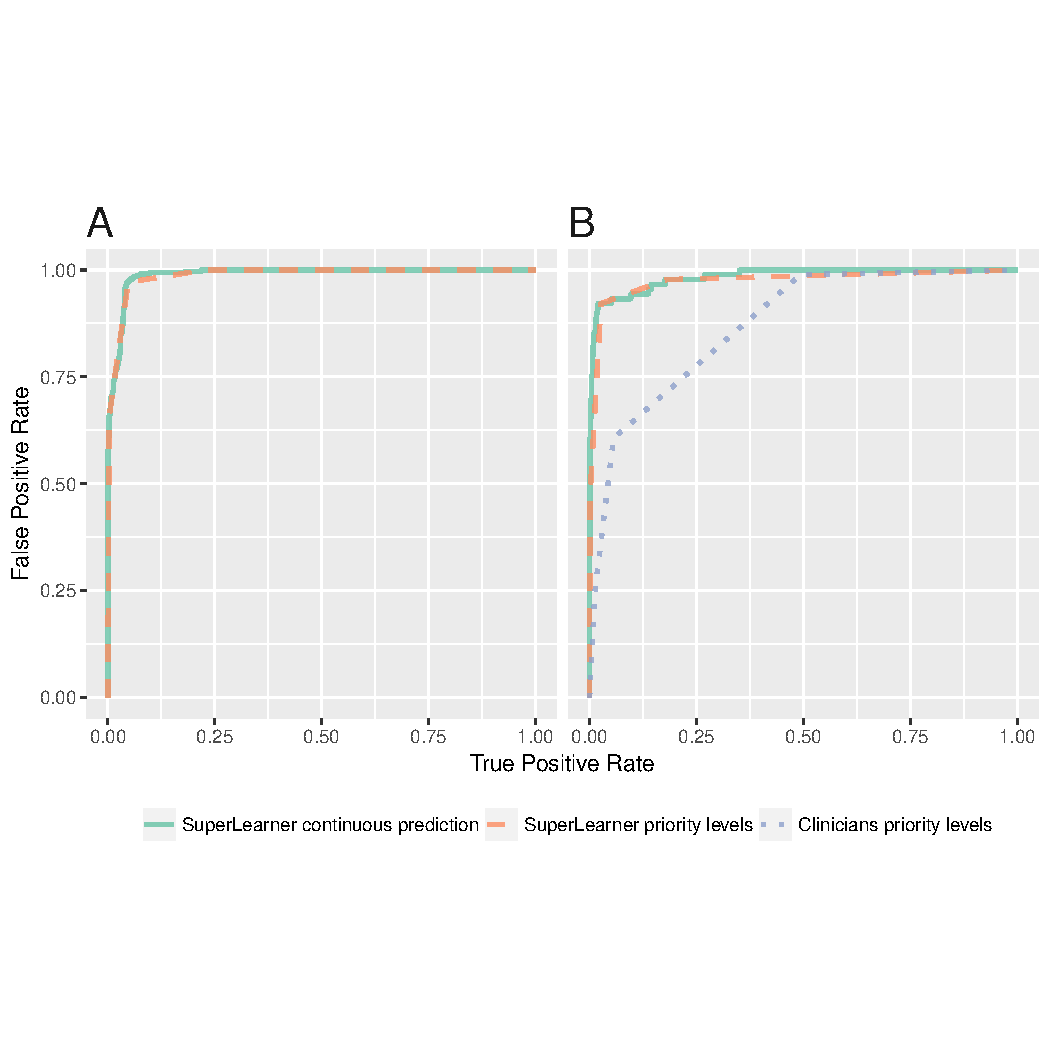
\includegraphics[width=\textwidth]{roc_plot.pdf}
\end{figure}

% *** Calibration plot
\begin{figure}
  \caption{Agreement between the continuous SuperLearner prediction and observed
    all cause 30-day mortality in the training (A) and test (B) samples.}
  \label{fig:calibration_plot}
  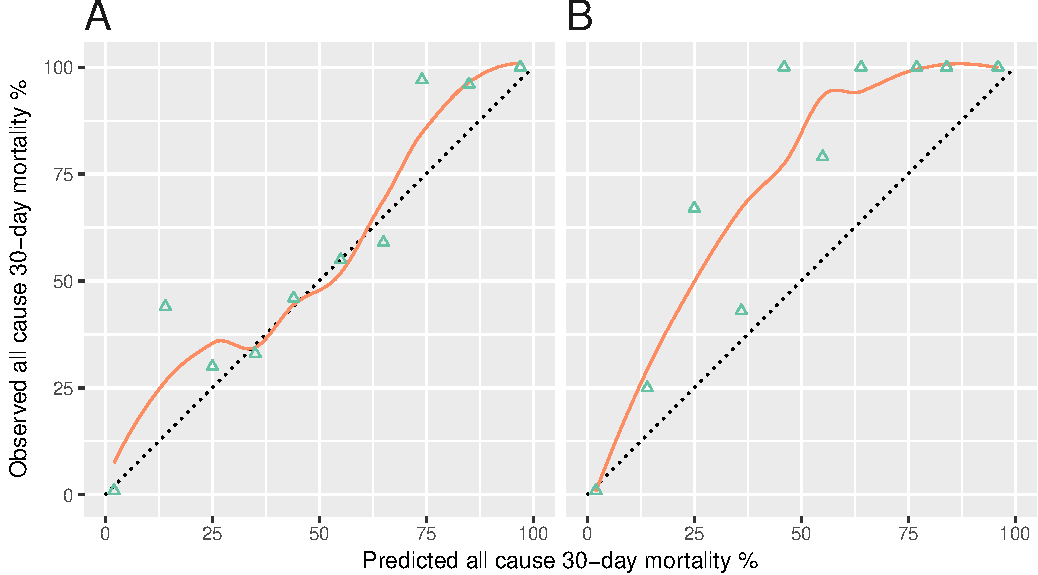
\includegraphics[width=\textwidth]{calibration_plot.pdf}
  \caption*{The straight dotted line indicates perfect agreement. The solid
    orange line is a smoothed association between mean mortality and mean
    predicted mortality across deciles of predicted mortality. The triangles are
    mortality point estimates across the same deciles.}
\end{figure}

% *** Mortality plot
\begin{figure}
  \caption{All cause 30-day mortality across priority levels in the test sample}
  \label{fig:mortality_plot}
  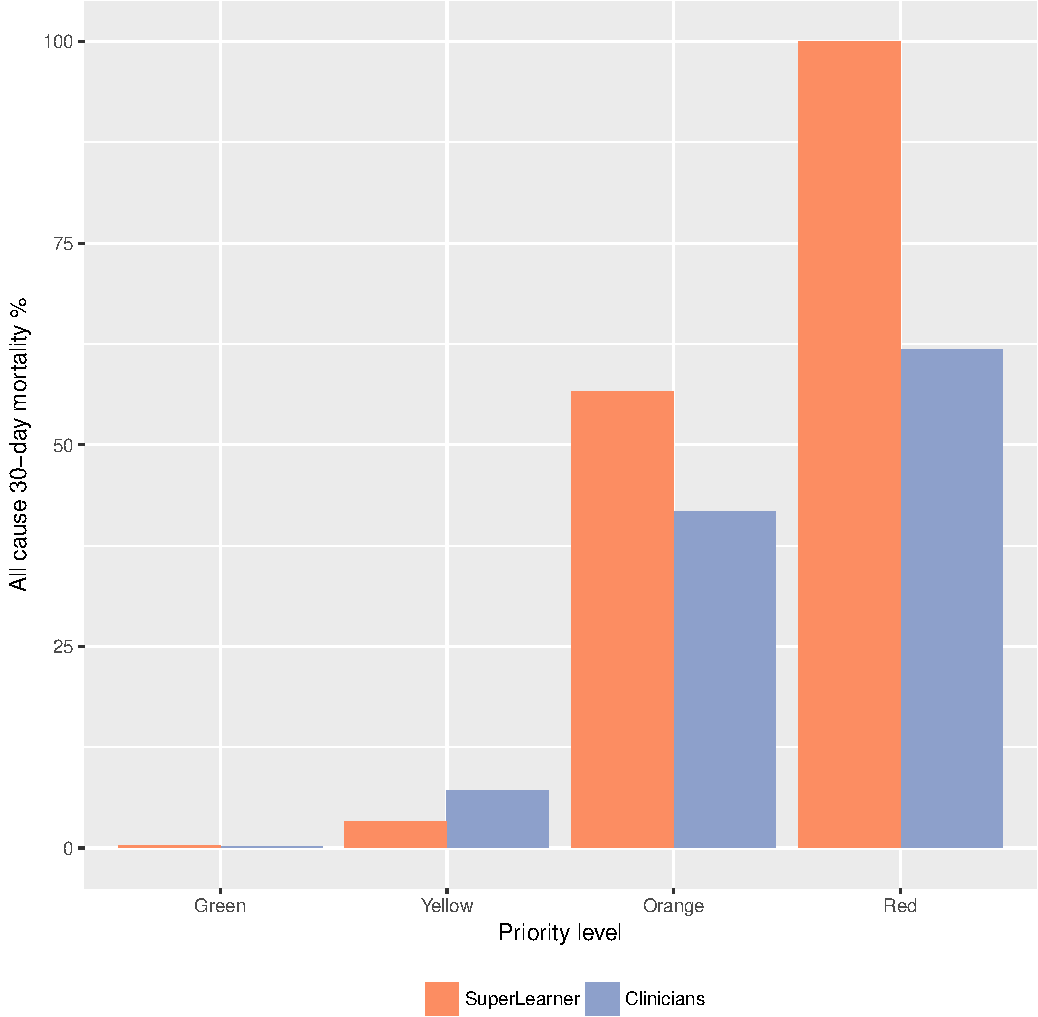
\includegraphics[width=\textwidth]{mortality_plot.pdf}
\end{figure}

% ** End document
\end{document}
